\documentclass[final,t]{beamer}
\usepackage{cmbright}
\usepackage[T1]{fontenc}
\usepackage{lipsum}  

%\usefonttheme[onlymath]{serif} %for math mode in serif

% poster template
\usepackage[orientation=portrait,scale=1.4,size=a0,debug]{beamerposter}
\setlength{\paperwidth}{48in}
\setlength{\paperheight}{36in}
\usetheme{zurichposter}

\definecolor{UMNgold}{RGB}{255,204,51}
\definecolor{UMNmaroon}{RGB}{122,0,25}

% references
\usepackage[bibstyle=authoryear, citestyle=authoryear-comp,%
hyperref=auto]{biblatex}
\bibliography{references}

% document properties
\title{\huge Operating Room Wireless Power Transfer System}
\author{\Large Cole Nielsen, Tri Phu, Sisay Weldegiorgis, Mason Tran, Alex Marvin\\\vskip1ex Advisors: Dr. Steven Koester \& Dr. Daniel Glumac}
\institute{\Large 6.78 MHz Resonant Inductive WPT using GaN-FET based Class-E Driver}
%------------------------------------------------------------------------------
\begin{document}

\begin{frame}{}
\begin{columns}[t]

\begin{column}{.02\paperwidth}
\end{column}


%-----------------------------------------------------------------------------
%                                                                     COLUMN 1
% ----------------------------------------------------------------------------

\begin{column}{.225\paperwidth}
	
	\begin{block}{Motivation \& Objective}
		\small Operating rooms (ORs) demand a high cost per minute during surgeries, approaching \$60-300 a minute. To lower costs, OR times should be shortened. Removal of power cables in OR allows this by reducing setup time for equipment such as X-Ray systems. This removal also offers other benefits, including increased mobility of equipment in the OR and improvement of safety by removing a major tripping hazard.\\\par\vskip1ex
		This project presents a solution to this problem by implementing a resonant-inductively coupled wireless power transfer system that could be implemented in ORs to replace cabled power.
	\end{block}	
	
    \vskip2.5ex
    
    \begin{center}
       	\includegraphics[width=\linewidth]{cart.png}
    \end{center}
    \FloatBarrier
	\vskip1ex
	
	\begin{exampleblock}{Solution \& Goals}
		\small Our solution is a resonant-inductive wireless power transfer system which consists of the following features (pictured above):
		\begin{itemize}
			\item[\textcolor{UMNmaroon}{\textbullet}] Transmitting coil array embedded in OR floor
			\item[\textcolor{UMNmaroon}{\textbullet}] Receiver coil mounted to cart, 4-8 inches from floor
			\item[\textcolor{UMNmaroon}{\textbullet}] 125 W power transfer ideal, >25W for demonstration
			\item[\textcolor{UMNmaroon}{\textbullet}] Compact (<1 ft$^2$)
			\item[\textcolor{UMNmaroon}{\textbullet}] Over power detection and shutdown
			\item[\textcolor{UMNmaroon}{\textbullet}] High-efficiency design
			\item[\textcolor{UMNmaroon}{\textbullet}] Compliance with government regulation (FCC)
		\end{itemize}
	\end{exampleblock}  
	\vskip2ex
	\begin{exampleblock}{Technical Approach - Architecture}
		\small Shown is the overall system architecture implemented.
		\begin{figure}[h!]
			\hspace*{-2.5ex}
			\resizebox{1\linewidth}{!}{% XCircuit output "block.tex" for LaTeX input from block.ps
\def\putbox#1#2#3#4{\makebox[0in][l]{\makebox[#1][l]{}\raisebox{\baselineskip}[0in][0in]{\raisebox{#2}[0in][0in]{\scalebox{#3}{#4}}}}}
\def\rightbox#1{\makebox[0in][r]{#1}}
\def\centbox#1{\makebox[0in]{#1}}
\def\topbox#1{\raisebox{-0.60\baselineskip}[0in][0in]{#1}}
\def\midbox#1{\raisebox{-0.20\baselineskip}[0in][0in]{#1}}
   \scalebox{1}{
   \normalsize
   \parbox{8.16667in}{
   \includegraphics[scale=1]{block.eps}\\
   % translate x=544 y=432 scale 0.38
   \tiny
   \putbox{1.81in}{0.97in}{1.20}{RF Power}%
   \putbox{5.31in}{0.97in}{1.20}{RF to DC}%
   \putbox{5.31in}{0.64in}{1.20}{Converter}%
   \putbox{7.31in}{0.81in}{1.20}{Load}%
   \putbox{1.81in}{0.64in}{1.20}{Generator}%
   \putbox{0.31in}{0.64in}{1.20}{Power}%
   \putbox{0.31in}{0.97in}{1.20}{Mains}%
   \putbox{3.89in}{0.06in}{1.20}{Coils}%
   } % close 'parbox'
   } % close 'scalebox'
   \vspace{-\baselineskip} % this is not necessary, but looks better
} 
				\end{figure}	
	 Major systems are:
		\begin{itemize}
			\item[\textcolor{UMNmaroon}{\textbullet}] RF generator: 6.78 MHz GaN Class-E power amplifier
			\item[\textcolor{UMNmaroon}{\textbullet}] Coil system: 4 coil resonant-inductive structure
			\item[\textcolor{UMNmaroon}{\textbullet}] RF to DC converter: Schottky bridge rectifier 
		\end{itemize}

	\end{exampleblock} 
	     	
	
\end{column}

\begin{column}{.02\paperwidth}
\end{column}

%-----------------------------------------------------------------------------
%                                                                     COLUMN 1
% ----------------------------------------------------------------------------

\begin{column}{.225\paperwidth}
	
	\begin{exampleblock}{Technical Approach - Coils}
		\small
		For high power transfer, a resonant-inductively (RI) coil system was chosen. Direct inductive coupling was found to have too low coupling in the desired range and coil size. The coil system was designed using a custom simulation code to extract coil inductance and coupling. The results for the implemented coil system, two 12" diameter coils separated 6", is shown:
		\vskip 1ex
		
	\begin{centering}
		\begin{tabular}{l r}
			\includegraphics[width=0.45\linewidth]{primary-field.png}	
		& 
			\includegraphics[width=0.45\linewidth]{secondary-field.png}
		\\
		\end{tabular} 
		\vskip 1ex
			\end{centering}	
		The extracted inductance and coupling parameters from the coil system simulation are below, where the corresponding circuit model is found below.
		\begin{equation}
			\nonumber k_{23} = 0.843 \hspace*{5ex} k_{12}=k_{34}=0.0909
		\end{equation}
		\begin{equation}
			\nonumber 		 L_{coil} = 944nH
		\end{equation}
		
			\vskip1ex
			\begin{center}
				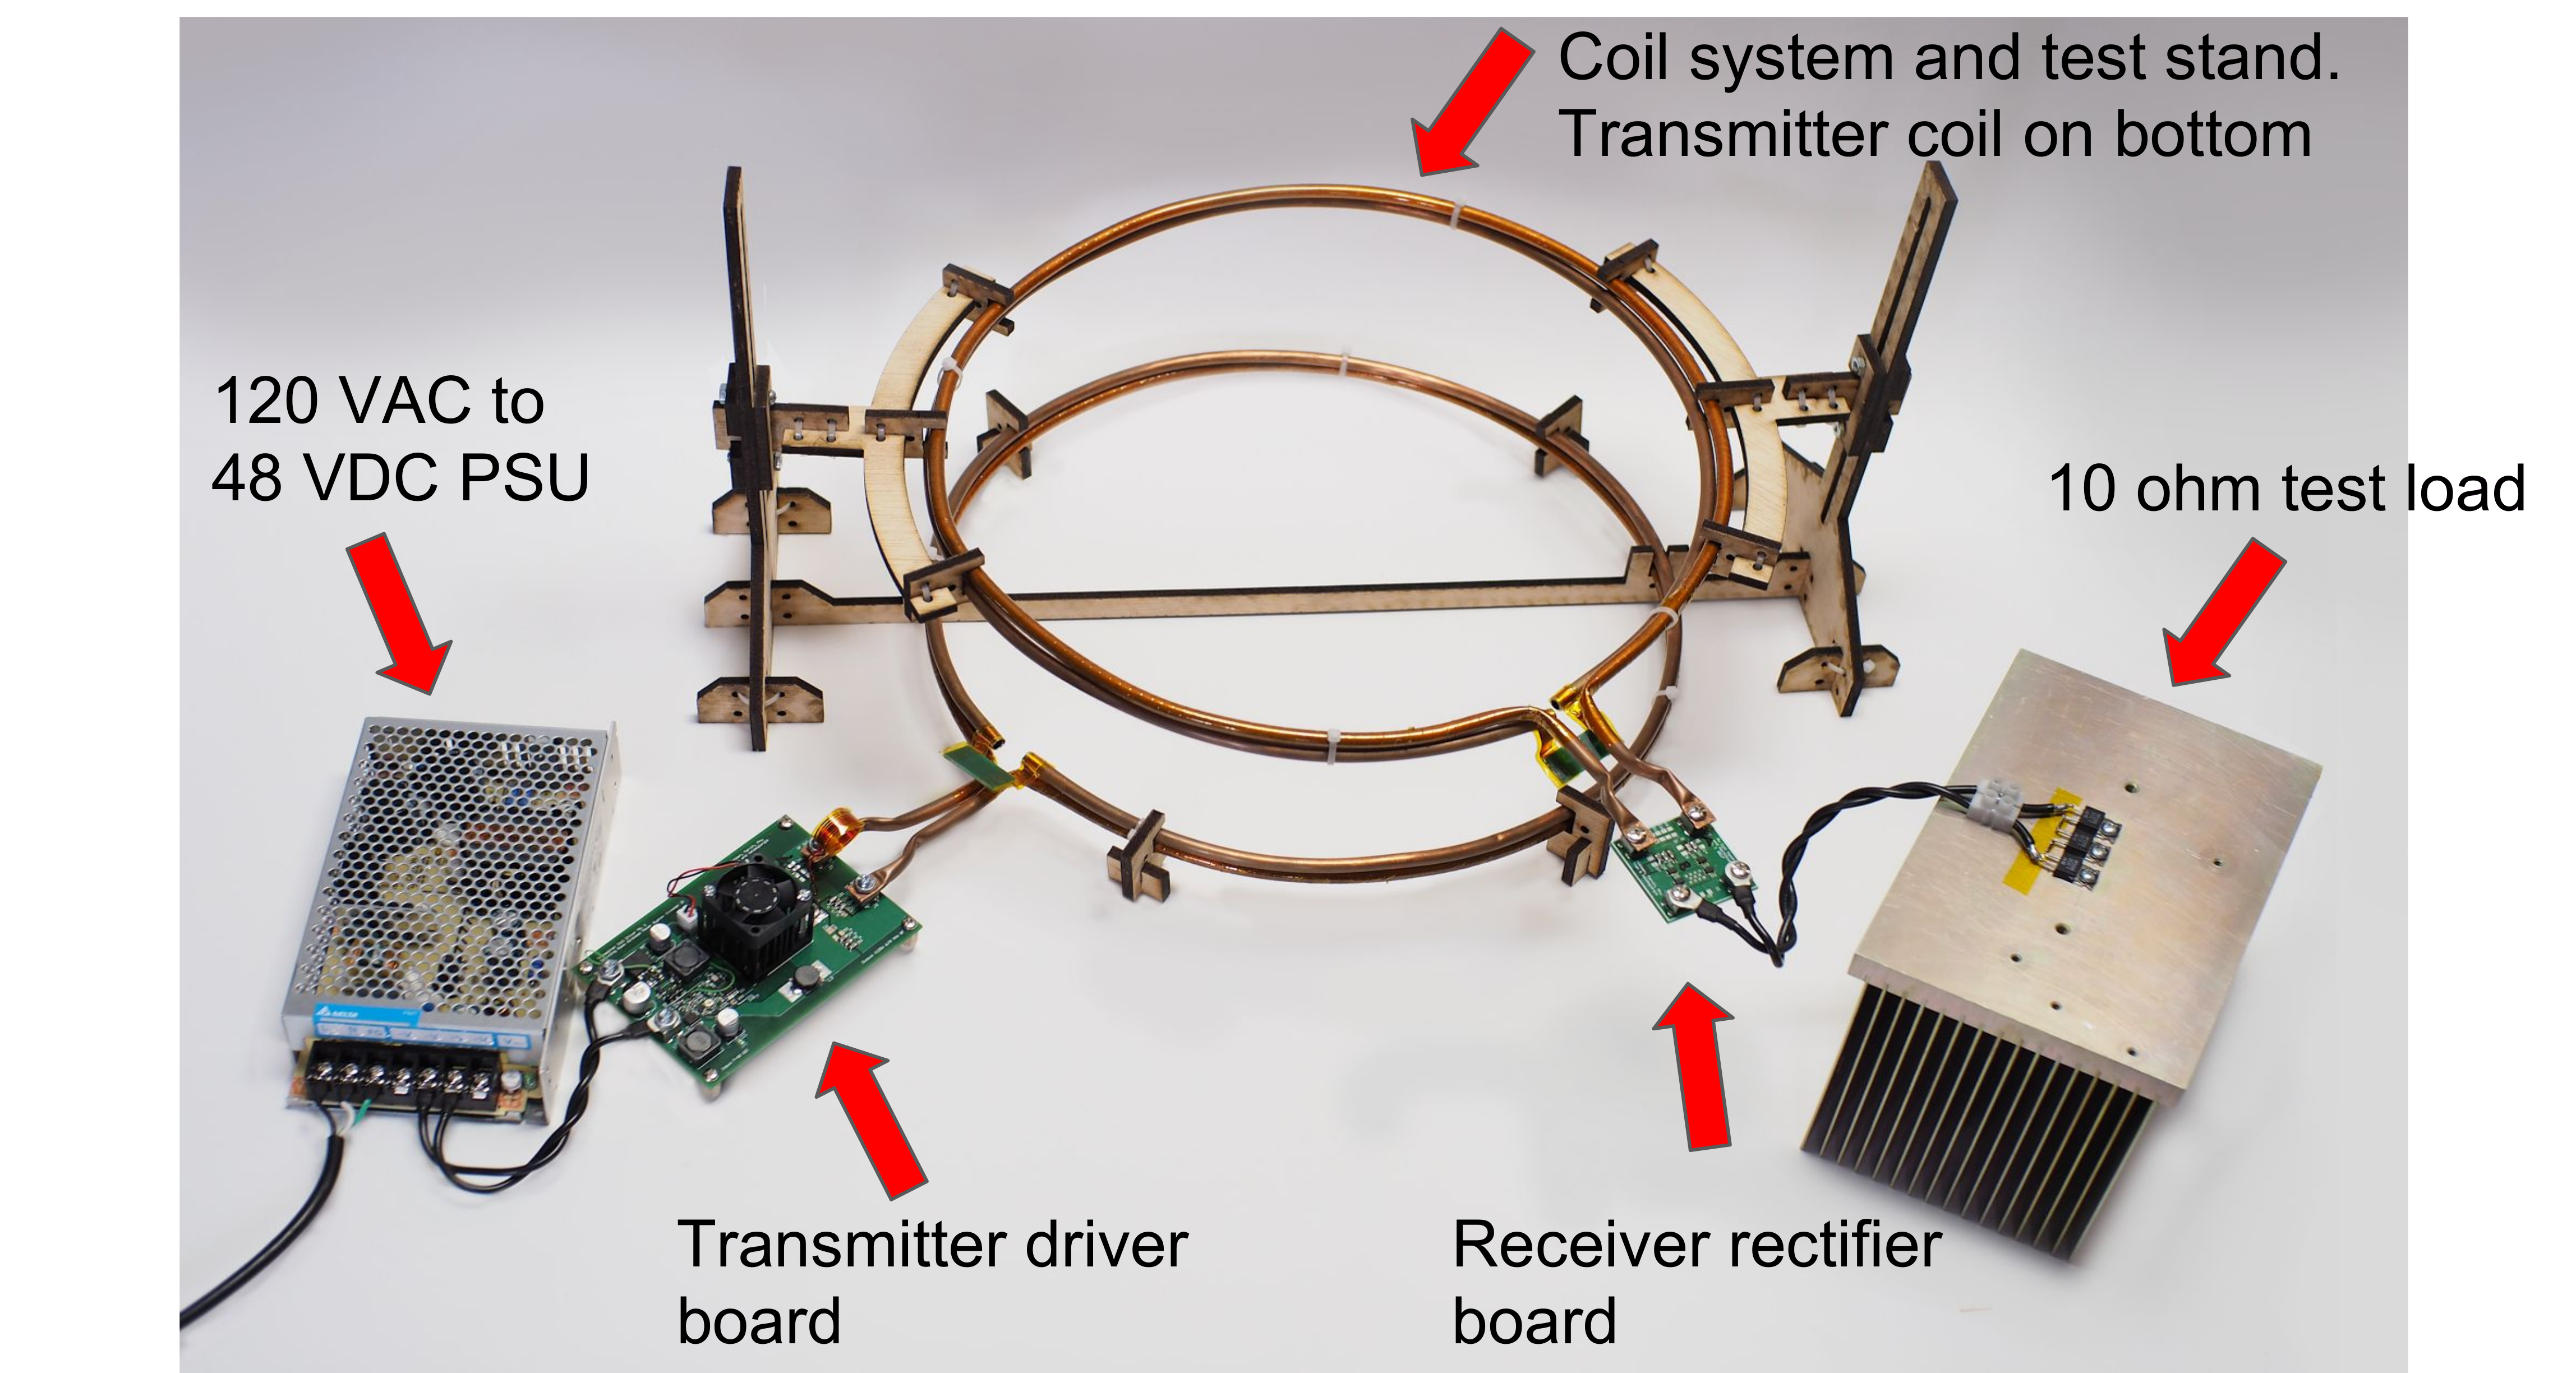
\includegraphics[width=\linewidth]{setup.png}
			\end{center}
			\FloatBarrier
			\vskip2ex
		
		The diagram below illustrates the structure of the 4-coil RI system, and the circuit model used for the coil system. Coil 1 is separated from 4 by 6", coil 2 is held within 0.25" of coil 1 as is coil 3 from coil 4.
			\begin{figure}[h!]
				\hspace*{-14ex}
				\resizebox{1.2\linewidth}{!}{% XCircuit output "circ.tex" for LaTeX input from circ.ps
\def\putbox#1#2#3#4{\makebox[0in][l]{\makebox[#1][l]{}\raisebox{\baselineskip}[0in][0in]{\raisebox{#2}[0in][0in]{\scalebox{#3}{#4}}}}}
\def\rightbox#1{\makebox[0in][r]{#1}}
\def\centbox#1{\makebox[0in]{#1}}
\def\topbox#1{\raisebox{-0.60\baselineskip}[0in][0in]{#1}}
\def\midbox#1{\raisebox{-0.20\baselineskip}[0in][0in]{#1}}
   \scalebox{0.5826}{
   \normalsize
   \parbox{10.6979in}{
   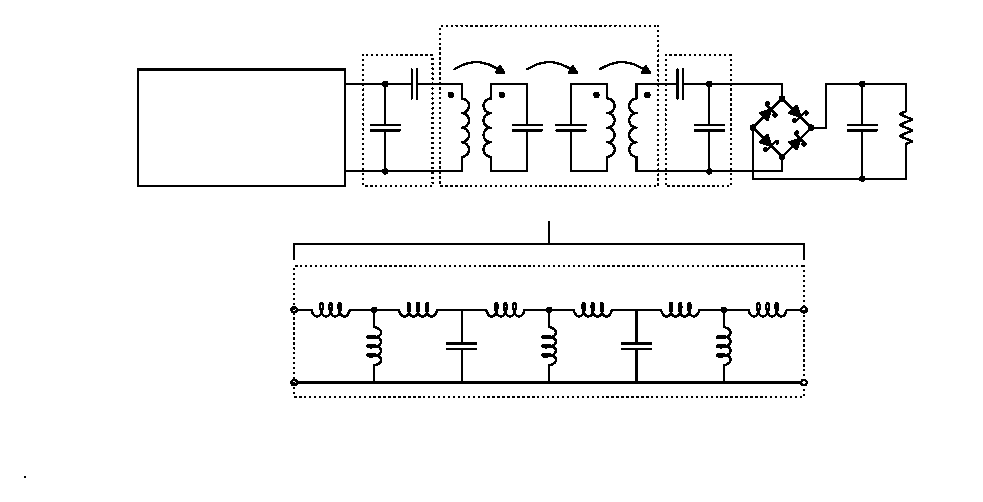
\includegraphics[scale=1.71644]{circ}\\
   % translate x=2193 y=969 scale 0.22
   \tiny
   \putbox{5.13in}{5.01in}{1.20}{k$_{12}$}%
   \putbox{5.93in}{5.01in}{1.20}{k$_{23}$}%
   \putbox{6.80in}{5.01in}{1.20}{k$_{34}$}%
   \putbox{2.09in}{4.34in}{1.20}{Class E }%
   \putbox{1.72in}{4.01in}{1.20}{Power Amplifer}%
   \putbox{1.43in}{3.68in}{1.20}{6.78 MHz RF Out}%
   \putbox{5.51in}{3.13in}{1.20}{Coil System}%
   \putbox{7.43in}{3.13in}{1.20}{Matching}%
   \putbox{3.93in}{3.13in}{1.20}{Matching}%
   \putbox{10.34in}{4.01in}{1.20}{Load}%
   \putbox{3.26in}{2.22in}{1.20}{(1-k$_{12}$)L}%
   \putbox{4.26in}{2.22in}{1.20}{(1-k$_{12}$)L}%
   \putbox{4.30in}{1.51in}{1.20}{k$_{12}$L}%
   \putbox{5.38in}{1.51in}{1.20}{C}%
   \putbox{5.26in}{2.22in}{1.20}{(1-k$_{23}$)L}%
   \putbox{6.26in}{2.22in}{1.20}{(1-k$_{23}$)L}%
   \putbox{7.26in}{2.22in}{1.20}{(1-k$_{34}$)L}%
   \putbox{8.26in}{2.22in}{1.20}{(1-k$_{34}$)L}%
   \putbox{7.38in}{1.51in}{1.20}{C}%
   \putbox{6.30in}{1.51in}{1.20}{k$_{23}$L}%
   \putbox{8.30in}{1.51in}{1.20}{k$_{34}$L}%
   \putbox{2.38in}{5.13in}{1.20}{Transmitter Side}%
   \putbox{8.09in}{5.09in}{1.20}{Receiver Side}%
   } % close 'parbox'
   } % close 'scalebox'
   \vspace{-\baselineskip} % this is not necessary, but looks better
} 
			\end{figure}
			\vskip-5ex
		Matching is performed using symmetric series-shunt capacitor networks on each side of the coil system, designed to present a real impedance on the primary side that equals that loading the secondary side (for this system Z$_L$ = 10 $\Omega$ was used). The middle image is the fully constructed coil system and electronics.
			
	\end{exampleblock}


	
\end{column}

\begin{column}{.02\paperwidth}
\end{column} 
%-----------------------------------------------------------------------------
%                                                                     COLUMN 2
% ----------------------------------------------------------- -----------------

\begin{column}{.225\paperwidth}
	
	\begin{exampleblock}{Technical Approach - Driver}
		\small For high efficiency, a Class-E power amplifier was designed to drive the coil system. Class-E amplifiers utilize zero voltage switching (ZVS) to minimize loses in the amplifier. The structure of a Class-E PA is shown below. The plot demonstrates ZVS operation, namely where the FET V$_{DS}$ and I$_D$ are exclusive, implying P$_{FET}$ = I$_D$V$_{DS}$ = 0.
		\begin{figure}[h!]
			\begin{center}
				\hskip-5ex
				\resizebox{1\linewidth}{!}{% XCircuit output "class-e-op.tex" for LaTeX input from class-e-op.ps
\def\putbox#1#2#3#4{\makebox[0in][l]{\makebox[#1][l]{}\raisebox{\baselineskip}[0in][0in]{\raisebox{#2}[0in][0in]{\scalebox{#3}{#4}}}}}
\def\rightbox#1{\makebox[0in][r]{#1}}
\def\centbox#1{\makebox[0in]{#1}}
\def\topbox#1{\raisebox{-0.60\baselineskip}[0in][0in]{#1}}
\def\midbox#1{\raisebox{-0.20\baselineskip}[0in][0in]{#1}}
   \scalebox{0.5826}{
   \normalsize
   \parbox{9.08333in}{
   \includegraphics[scale=1.71644]{class-e-op}\\
   % translate x=345 y=905 scale 0.22
   \putbox{2.09in}{2.26in}{1.20}{Amplifier Output}%
   \putbox{2.43in}{2.01in}{1.20}{Network}%
   \putbox{1.01in}{2.09in}{1.20}{RFC}%
   \putbox{0.09in}{1.09in}{1.20}{Gate}%
   \putbox{0.09in}{0.84in}{1.20}{Drive}%
   \putbox{0.59in}{0.18in}{1.20}{Gate Drive}%
   \putbox{4.18in}{1.09in}{1.20}{Load}%
   \putbox{6.01in}{2.59in}{1.20}{Vds}%
   \putbox{7.68in}{2.34in}{1.20}{Id}%
   \putbox{6.76in}{0.09in}{1.20}{Time}%
   \putbox{1.59in}{2.84in}{1.20}{48V}%
   } % close 'parbox'
   } % close 'scalebox'
   \vspace{-\baselineskip} % this is not necessary, but looks better
} 
			\end{center}
		\end{figure}
			The above structure was implemented utilizing a Gallium Nitride (GaN) FET as the switch. GaN was chosen due to the relatively high 6.78 MHz system frequency (done to take advantage of relaxed FCC regulation of ISM bands), low loss required and high switching node voltages, of which only GaN devices can satisfy. The load in this circuit would be the coil network. The below image shows the Class-E power amplifier board constructed for this project.
	\end{exampleblock}

	\vskip2cm
	\begin{center}
		\includegraphics[width=\linewidth]{board-labeled.jpg}
	\end{center}
	\FloatBarrier
	\vskip2ex
	
	\begin{exampleblock}{Implementation}
		\small The described system was implemented as shown in the images above and to the left. The power amplifier and receiving side rectifier were implemented on their own PCBs respectively, the coils were constructed out of 0.25" copper tubing and mounted into a custom laser cut testing stand, adjustable in coil separation.\\
		\vskip1ex
		A 10 $\Omega$ load was constructed for testing out of three 3.3 $\Omega$ thin film resistors on a large heat sink, permitting up to 150W of power dissipation with minimal parasitic capacitance.
	\end{exampleblock}
	
\end{column}

\begin{column}{.02\paperwidth}
\end{column}

%-------------------------------------------------------------
%                                                                     COLUMN 2
% ----------------------------------------------------------------------------
\begin{column}{.225\paperwidth}

		\begin{exampleblock}{Testing \& Performance Results}	
		\small Testing was performed by adjusting the coil separation at various supply voltages until maximum transfer was observed. Power at the load is P$_L$ = $\frac{V_L^2}{R_L}$, and input power is P$_{in}$ = $I_{in}V_{in}$. The best result for power transfer is shown below:
		\begin{center}
			\includegraphics[width=0.63\linewidth]{highest-power2.png}
		\end{center}
		\FloatBarrier
	Max transfer was with V$_L$ = 22.8V$_{RMS}$ into a 10.3 $\Omega$ load, while drawing 2.16A at 36V from the supply. This corresponds to:
		\begin{equation}
			\nonumber P_{transfer} = 50.5W \hskip5ex \eta = \frac{P_L}{P_{in}} = 64.6 \%
		\end{equation}
		This satisfies >25W power transfer. The spectrum of the output of the driver board was also measured to verify compliance to FCC regulations for the 6.78 MHz ISM band. 
			\begin{center}
				\includegraphics[width=0.63\linewidth]{spectrum2.png}
			\end{center}
			\FloatBarrier
			As seen in the above plot, the signal is centered at 6.78 MHz with visible sidebands extending to $\pm$ 5KHz. This is well within the 6.78 MHz $\pm$ 15 KHz allocated by the FCC for the first ISM band. 
		\end{exampleblock}
		\vskip1ex
	
	\begin{alertblock}{Conclusions}	
	\small A prototype wireless power system was successfully developed demonstrating non-trivial (>50W) power transfer wirelessly. The system also maintained dimensional constraints and compliance to government regulation. These factors combined imply the success of the project in addition to its viability to be further developed in future semesters.
		\end{alertblock}
		\vskip 1ex
				% References
		\begin{block}{Future Work}
			\small Given the possibility of the continuation of this project, numerous aspects of this design can yet be improved and expanded upon. For example:

		\begin{itemize}
				\item[\textcolor{UMNmaroon}{\textbullet}] Development of a receiver-side power converter to deliver 120 VAC to devices
				\item[\textcolor{UMNmaroon}{\textbullet}] Development of a multi-transmitter coil array
				\item[\textcolor{UMNmaroon}{\textbullet}] Receiver integration onto medical cart
		\end{itemize} 
		\end{block}
				
				
			\end{column}

\end{columns}

\end{frame}

\end{document}
